% this file is called up by thesis.tex
% content in this file will be fed into the main document

\chapter{Consideration} % top level followed by section, subsection


% ----------------------- paths to graphics ------------------------

% change according to folder and file names
\ifpdf
    \graphicspath{{7/figures/PNG/}{7/figures/PDF/}{7/figures/}}
\else
    \graphicspath{{7/figures/EPS/}{7/figures/}}
\fi


\section{Design for Manufacter}

The current prototype is only suitable for simulation. Several changes are
necessary for real world applications. Firstly, addition to the NVMe command set
in the form of a new NVMe namespace. Secondly, the ABI needs to be formalized
and become a integral part of the specification. Third, existing drivers, such
as SPDK or xNVME, must be updated to support this new namespace and commands.

% Describe how the design would change for a real world, practical
% implementation. Take the ICD loader diagram as base.

\begin{figure}
    \centering
	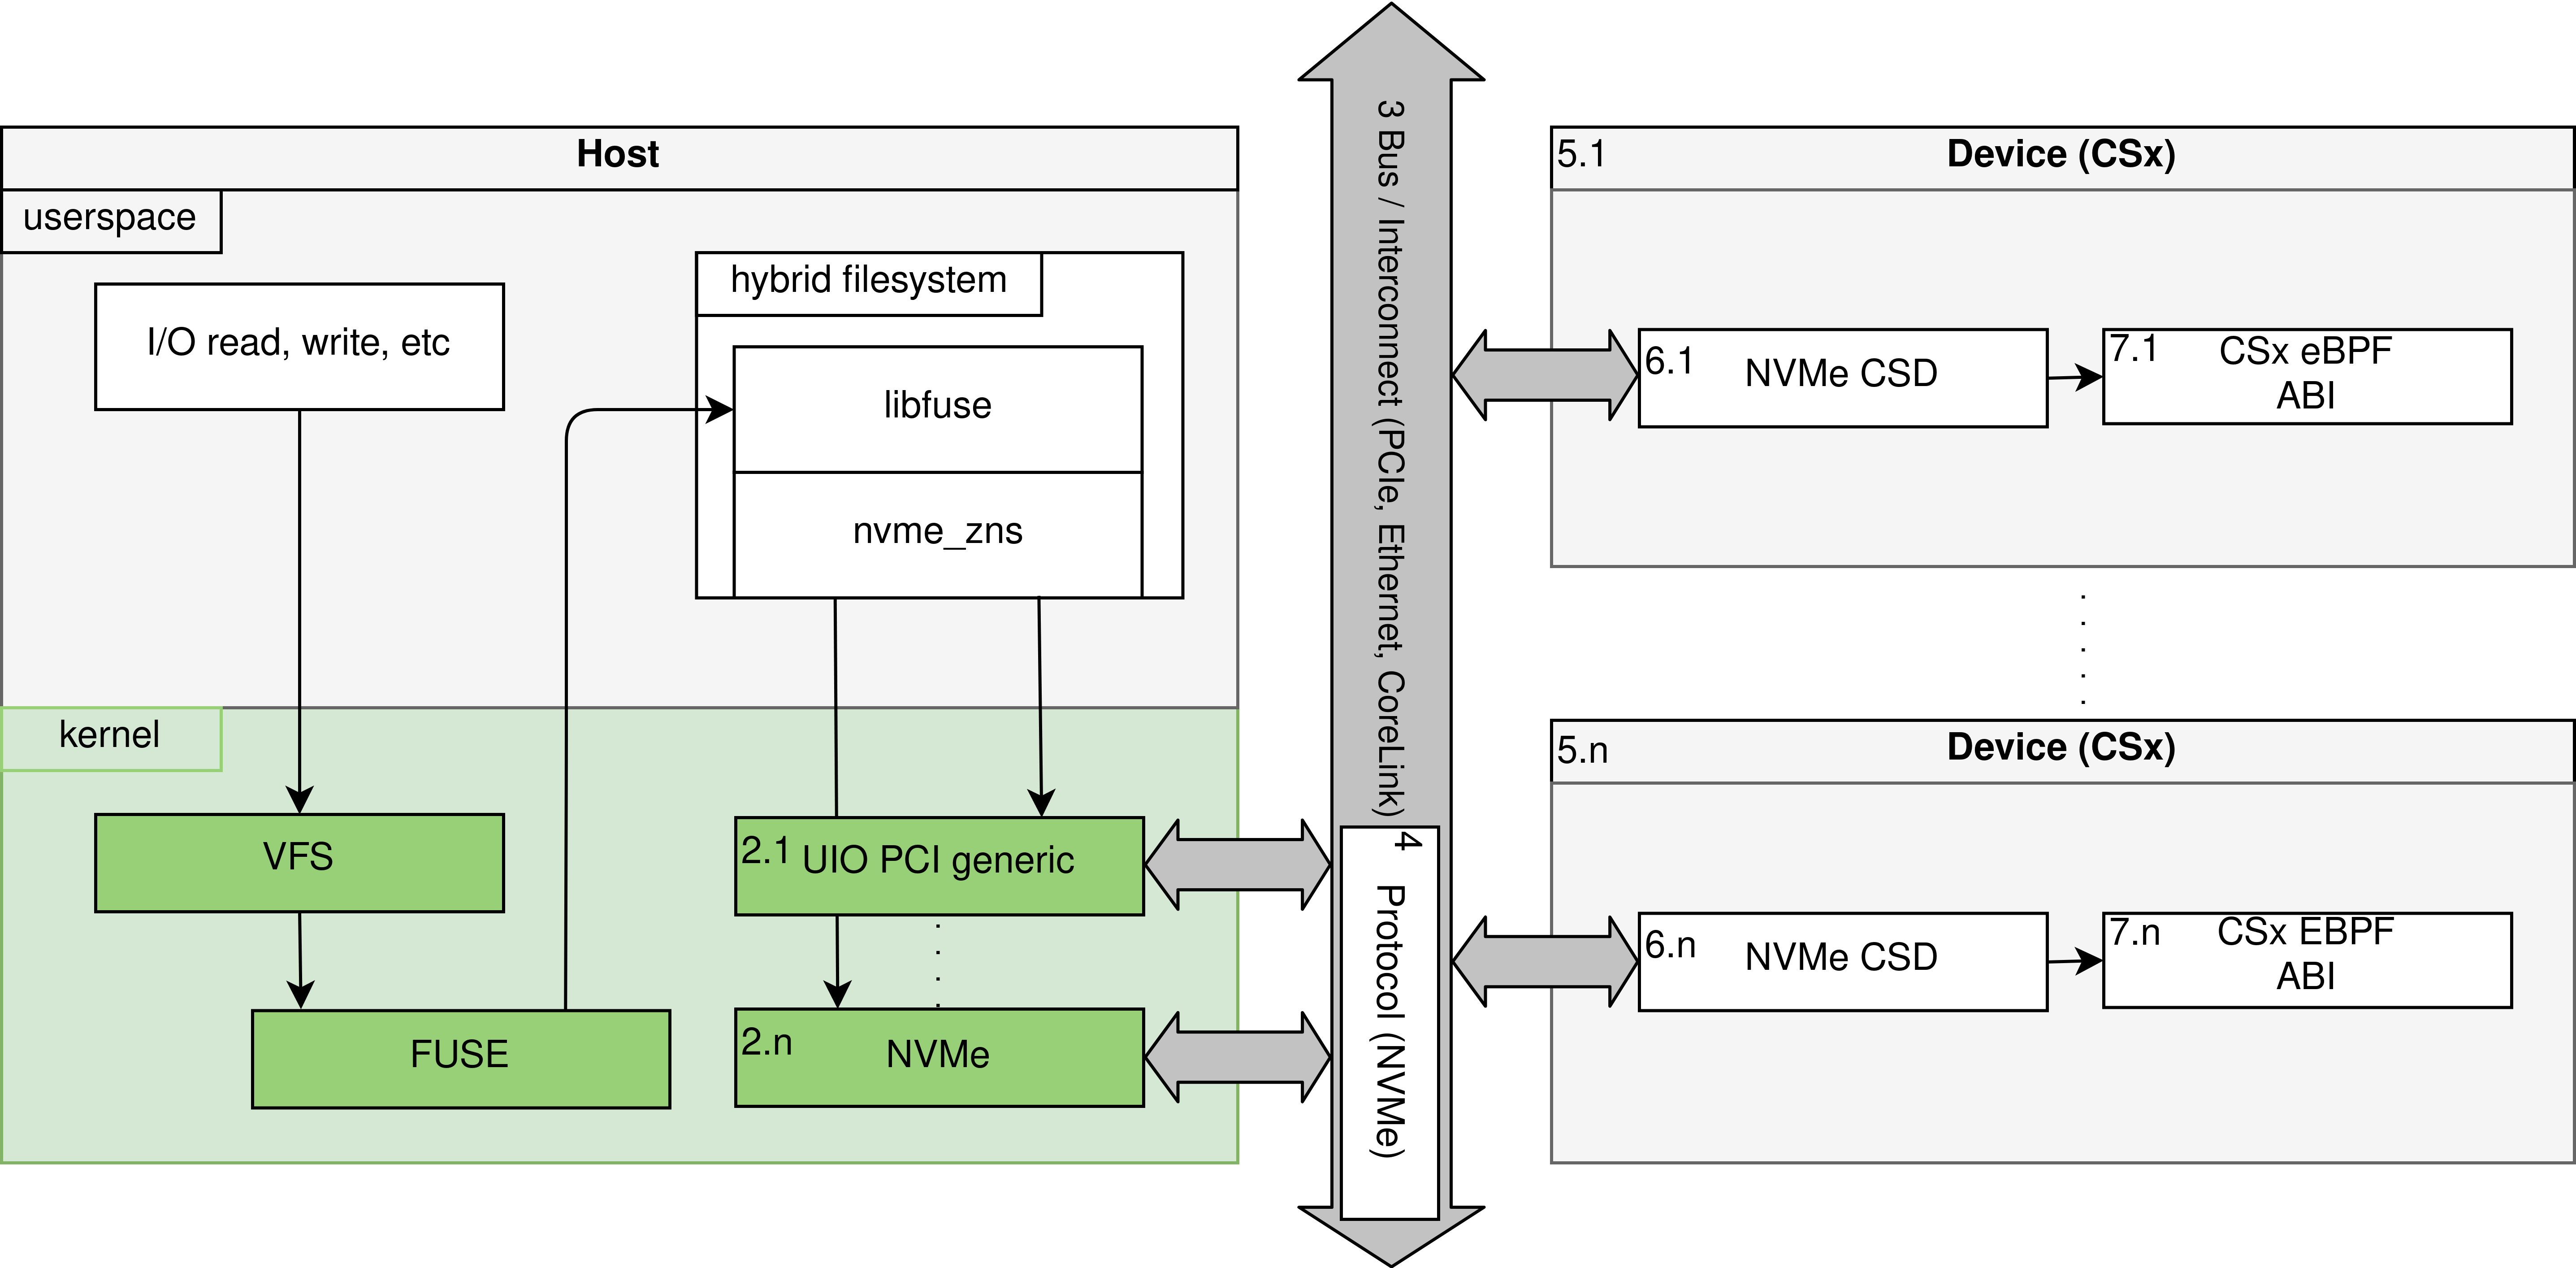
\includegraphics[width=1\textwidth]{resources/images/loader-pfs-arch-v3.png}
	\caption{Practical complete architecture for vendor agnostic CSxs with
        potential filesystem support.}
    % \includesvg[width=0.6\columnwidth]{resources/images/module-dependencies}
    \label{figure:practicalarchitecture}
\end{figure}

Use statfs to determine the type of filesystem, ICDs are related to a specific
filesystem type. The CSx eBPF ABI should contain atleast one system call to
retrieve the vendor filesystem context data for the current request (already
part of prototype). The CSx FS API contains functions and datastructures to
allow the kernel to transform this context data. The API is implemented by
individual filesystems as shared library and made available throught the ICD.
The CSx FS runtime uses a loader with mechanisms such as \textit{dlopen} to
verify the contents of the provided library in accordance to the API.

The basic format of the ICD can be extended such that it could support
extensions to the base API as well as contain versioning. Typically, ICD files
are human readable using a markup language such as YAML. This is same approach
as the prominent video graphics API Vulkan.

\begin{figure}
    \centering
	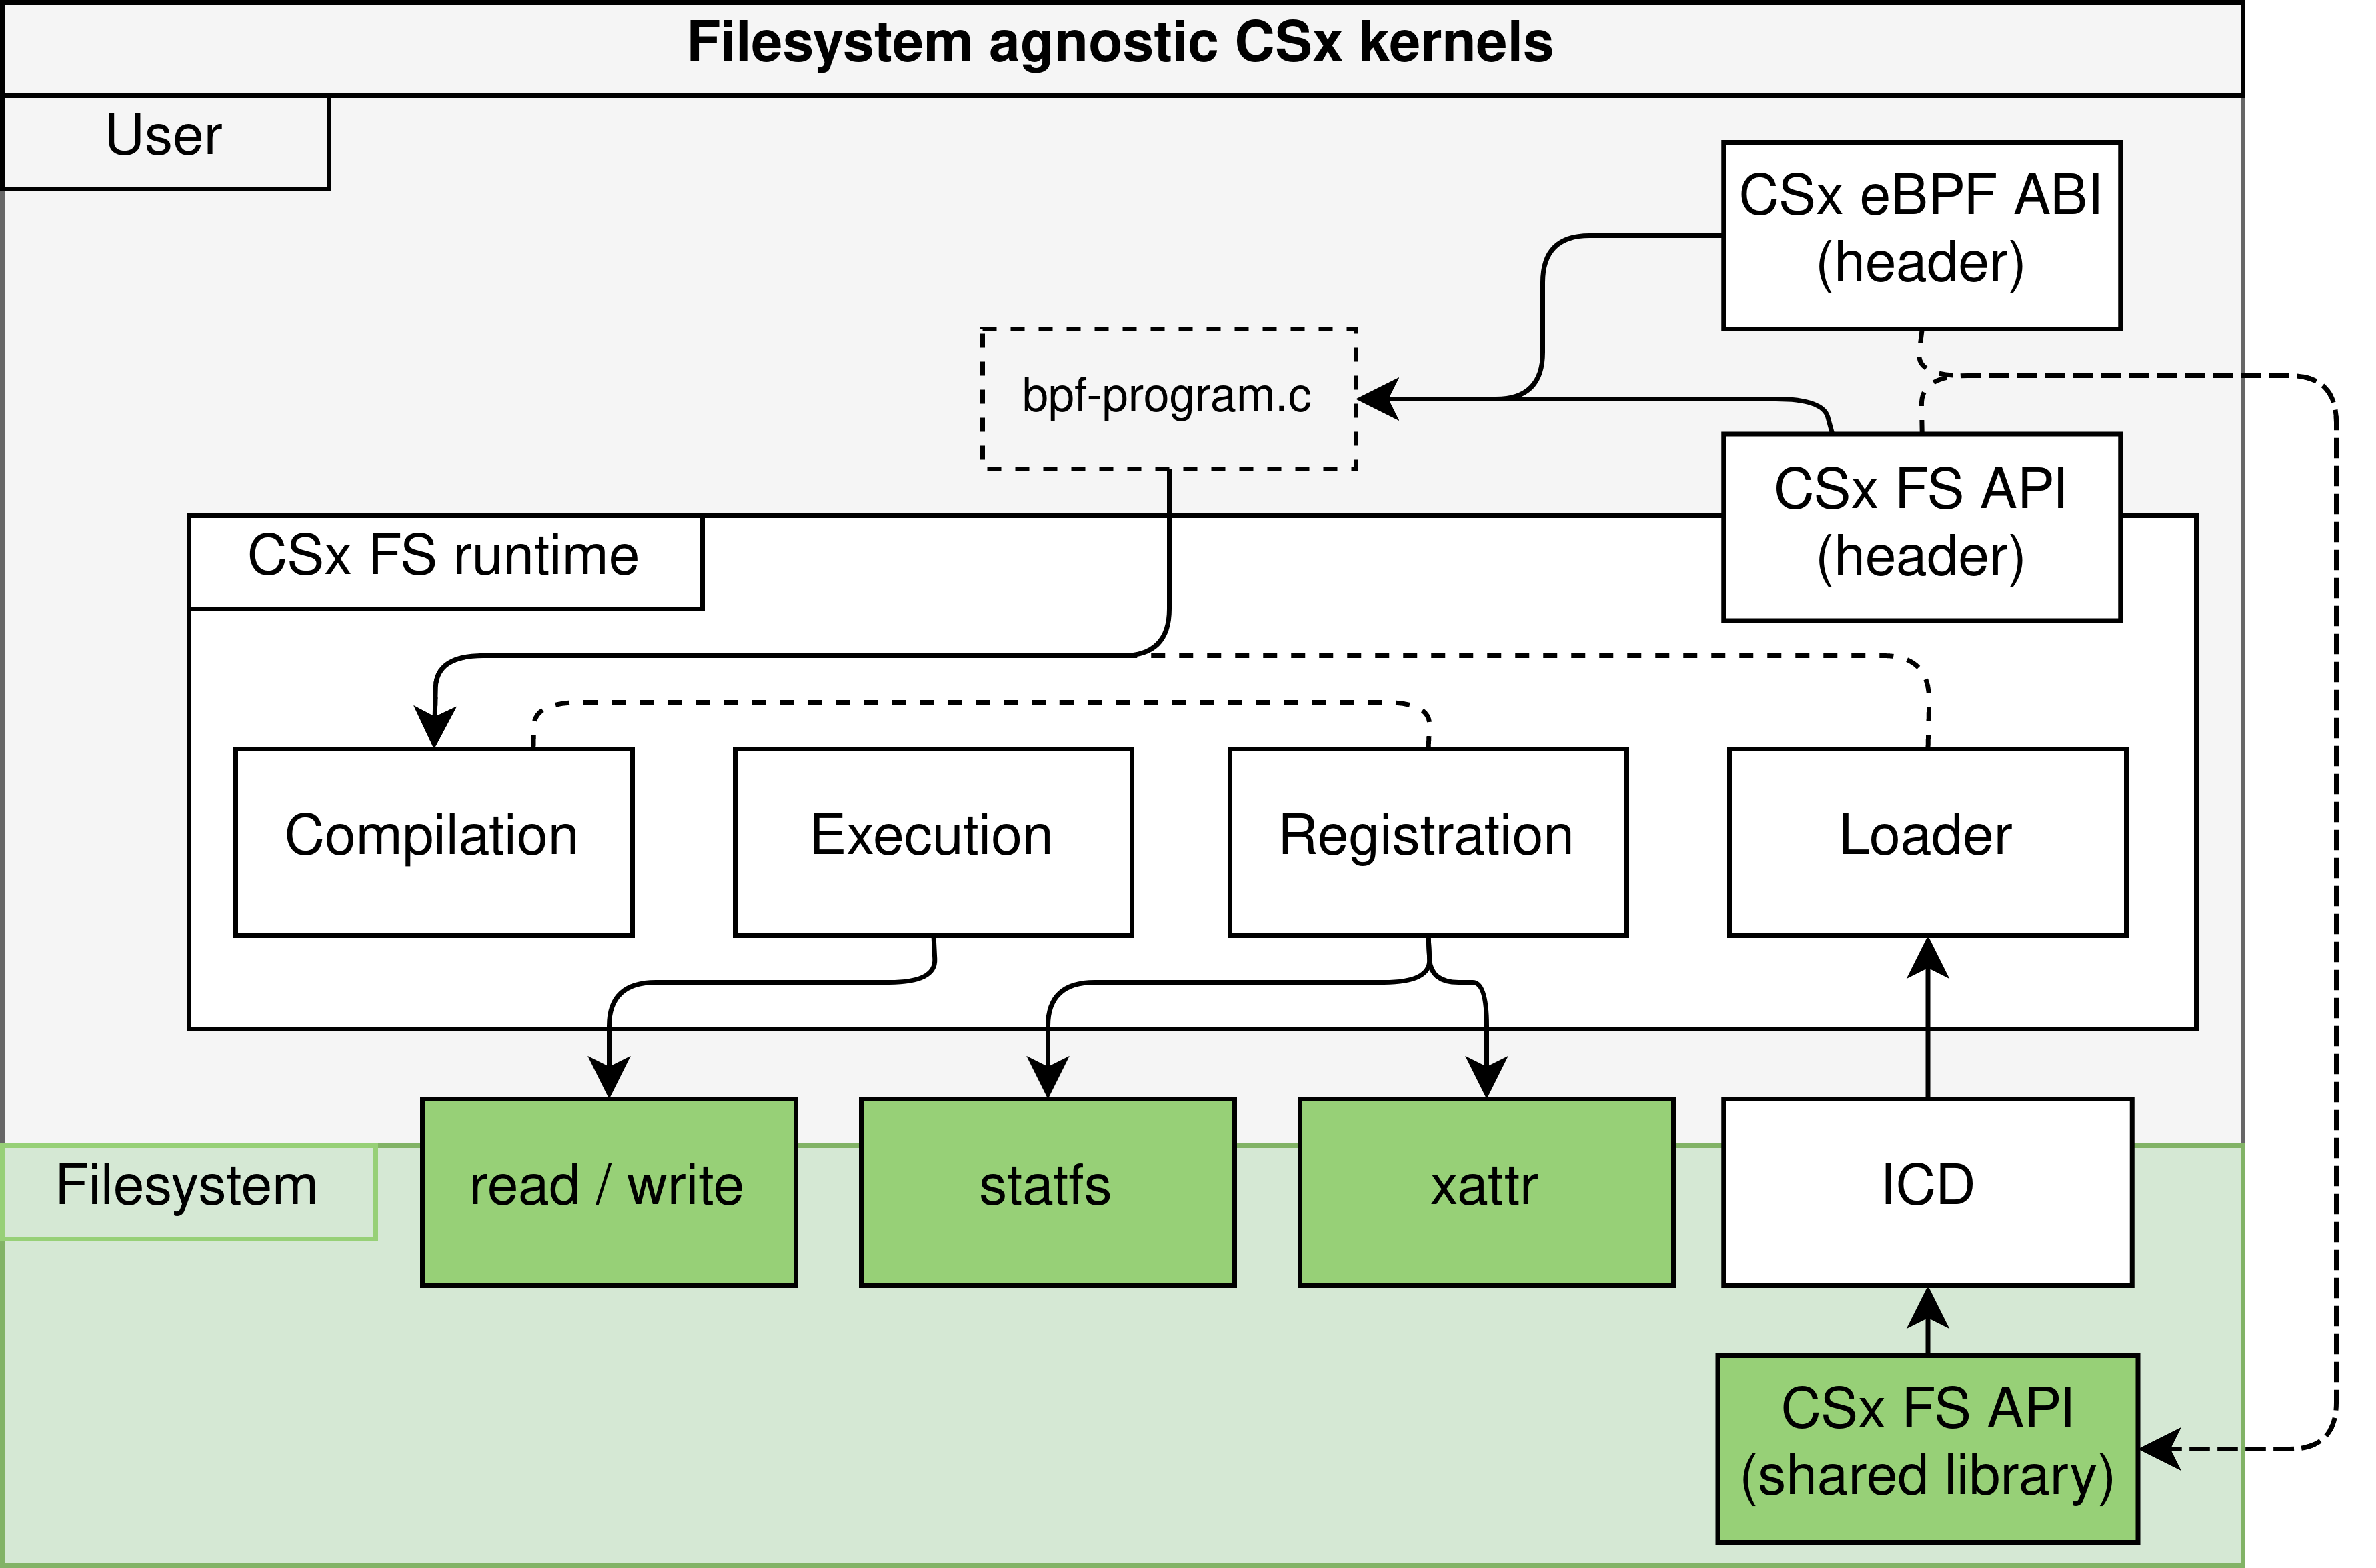
\includegraphics[width=0.7\textwidth]{resources/images/csx-fs-agnostic.png}
	\caption{Extended architecture to support filesystem agnostic CSx kernels.}
    % \includesvg[width=0.6\columnwidth]{resources/images/module-dependencies}
    \label{figure:csxfsruntime}
\end{figure}


% ---------------------------------------------------------------------------
% ----------------------- end of thesis sub-document ------------------------
% ---------------------------------------------------------------------------